\documentclass{article}
\usepackage{tikz}
\usetikzlibrary{arrows.meta, positioning}

\begin{document}

\begin{figure}[h]
    \centering
    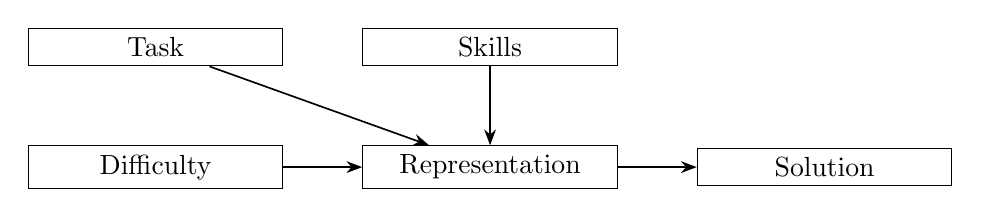
\begin{tikzpicture}[
        node distance = 10mm and 10mm,
         box/.style = {draw, text width=3cm, align=center},
         arr/.style = {-Stealth, semithick}
        ]
        \node (task) [box] {Task};
        \node (skills) [box, right=of task] {Skills};
        \node (representation) [box, below right=of task] {Representation};
        \node (solution) [box, right=of representation] {Solution};
        \node (difficulty) [box, left=of representation] {Difficulty};

        \draw[arr] (task) -- (representation);
        \draw[arr] (skills) -- (representation);
        \draw[arr] (representation) -- (solution);
        \draw[arr] (difficulty) -- (representation);
    \end{tikzpicture}
    
    \caption{Flowchart of Problem-Solving Process}
    \label{fig:flowchart}
\end{figure}

Alice was beginning to get very tired of sitting by her sister on the bank, and of having nothing to do: once or twice she had peeped into the book her sister was reading, but it had no pictures or conversations in it, ``and what is the use of a book,'' thought Alice ``without pictures or conversations?''

So she was considering in her own mind (as well as she could, for the hot day made her feel very sleepy and stupid), whether the pleasure of making a daisy-chain would be worth the trouble of getting up and picking the daisies, when suddenly a White Rabbit with pink eyes ran close by her.

\end{document}